% !TEX root=../../report.tex

\Section{Anwendungsfälle}
\label{ucSection}

Aus einer groben Idee werden in Planungsrunden, bei denen das ganze Team anwesend ist, einige Anforderungen definiert. Diese Anforderungen lassen sich in sogenannte Muss- und Kann-Anforderungen unterteilen. Erstere müssen umgesetzt werden, da sonst das Konzept des Systems nicht abgebildet, die Sicherheit gefährdet, oder die Benutzerfreundlichkeit vernachlässigt wird. Letztere können bearbeitet werden. Sie sind aus weiterführenden Diskussionen entstanden und können den Anwender bei bestimmten Arbeitsschritten weiter unterstützen.

Die Anforderungen werden in einem \gls{uml} Use-Case Diagramm festgehalten.

\begin{figure}[ht]
\centering
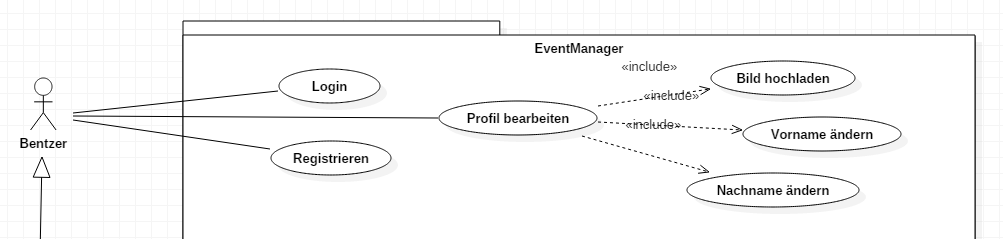
\includegraphics[width=\textwidth]{res/images/UseCaseUser.png}
\caption{Grundlegende Anwendungsfälle}
\label{uc1}
\end{figure}

Die grundlegenden Anforderungen eines Benutzers an das System werden in \myautoref{uc1} dokumentiert. So soll sich ein Benutzer an der Plattform registrieren können. Für ihn wird dann ein Benutzerkonto angelegt, welches auch personalisiert werden soll. Die benötigten Informationen hierbei sind die EMail Adresse, der Vorname und der Nachname. Optional soll noch ein Profilbild hinterlegt werden können. Um mit dem System arbeiten zu können, muss eine Möglichkeit geschaffen werden, sich mit einer EMail-Passwort Kombination anzumelden. Alle weiteren Akteure im Use-Case Diagramm erben diese Anforderungen. \newpage

\begin{figure}[ht]
\centering
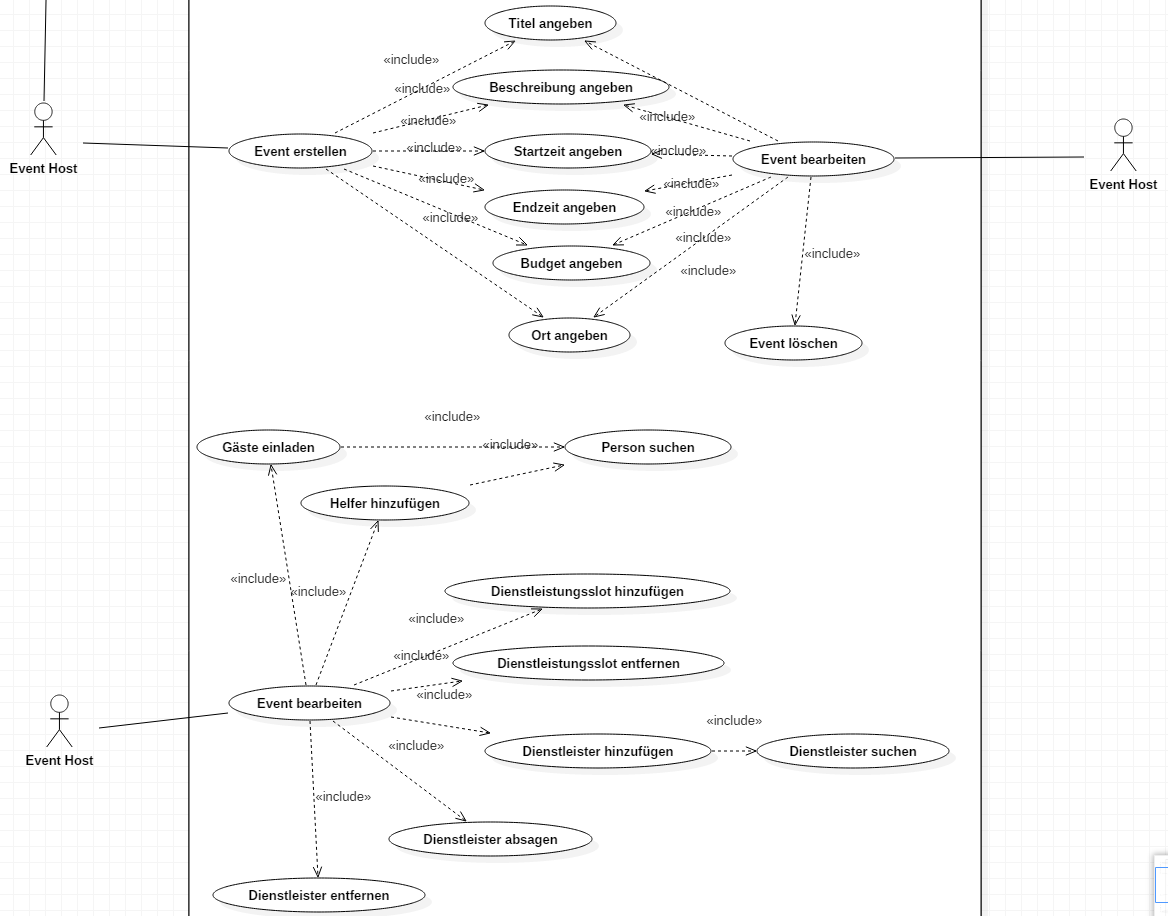
\includegraphics[width=\textwidth]{res/images/UseCaseEventHost.png}
\caption{Anforderungen eines Veranstalters an das System}
\label{uc2}
\end{figure}

Die \myautoref{uc2} beschreibt die Anforderungen eines Event\-erstellers an das System. Diese behandeln das Erstellen, sowie das Bearbeiten einer Veranstaltung. In beiden Fällen sollen die erforderlichen Informationen wie Titel, Start- und Endzeit bearbeitet werden können. Auch sollen die optionalen Felder, wie die Beschreibung, das vorgesehene Budget, und der Veranstaltungsort ebenfalls editierbar sein.

Besteht der Wunsch, dass die Veranstaltung nicht mehr angeboten wird, soll außerdem eine Möglichkeit des Löschens vorgesehen werden.

Nachdem nun das Event mit seinen grundlegenden Eigenschaften erstellt werden kann, geht es jetzt darum, die Dienstleister anzufragen. Für diesen Zweck sind die Serviceslots vorgesehen. Diese sollen mit den erforderlichen Parametern, wie der Start- und Endzeit, der Servicekategorie und der Preisvorstellung angelegt und bearbeitet werden können. Der Slot benötigt zusätzlich eine Funktion, um nach Anbietern zu suchen. Die gefundenen Dienstleister entsprechen der Kategorie des zugehörigen Slots. Damit Flexibilität ermöglicht wird, müssen zugeordnete Anbieter auch wieder aus den Serviceslots gelöscht werden können.

Für die Gästeplanung müssen auch Gäste eingeladen werden. Hierfür soll eine Suche über die registrierten Benutzer ermöglicht werden. Es gibt die Möglichkeit, dass der Veranstalter bestimmte Gäste zu Helfern ernennt. Auch die Helfer müssen von der Suche gefunden werden können.

\begin{figure}[h]
\centering
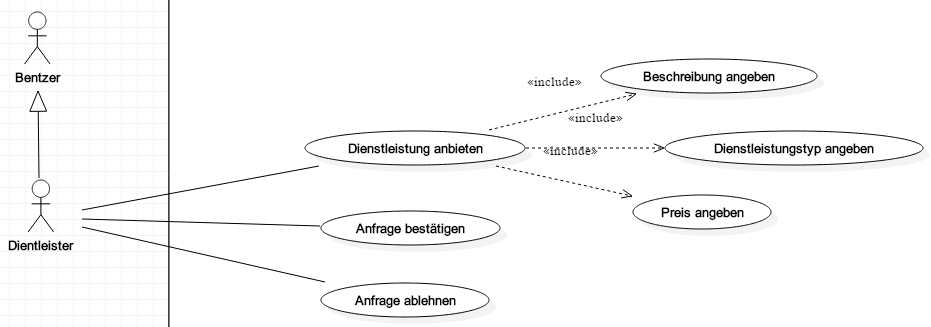
\includegraphics[width=\textwidth]{res/images/UseCaseServiceProvider.png}
\caption{Anwendungsfälle der Dienstleister}
\label{uc3}
\end{figure}

Ein Dienstleister will auf der Plattform seinen Service abieten, wie in \myautoref{uc3} festgehalten. Dazu muss eine Dienstleistung angeboten und auch wieder geändert werden können. Eine Dienstleistung muss eine Beschreibung, sowie eine Preisvorstellung besitzen. Für die Filterfunktion des Event Managers wird eine Information über die Kategorie der Leistung benötigt. Besteht der Wunsch, diese Dienstleistung nicht mehr anzubieten, so muss sie wieder gelöscht werden können.

Wird ein Dienstleister mit seinem Angebot zu einem Serviceslot hinzugefügt, muss diese Anfrage beantwortet werden, um Rückmeldung über den Status zu geben.

\begin{figure}[h]
\centering
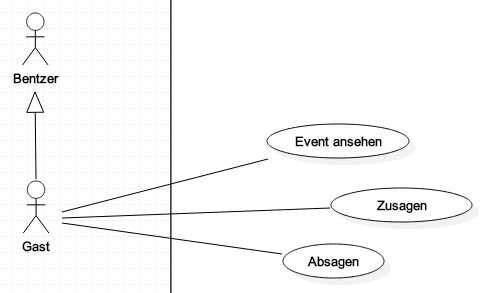
\includegraphics[width=.5\textwidth]{res/images/UseCaseGuest.png}
\caption{Use-Cases eines Gastes}
\label{uc4}
\end{figure}

Für den Gast ist es von großer Bedeutung, die Details der Veranstaltung einsehen zu können, für welche er eingeladen wurde. Um dem Veranstalter die Planung zu erleichtern, soll signalisiert werden können \enquote{Ja, ich werden teilnehmen}, oder auch \enquote{Nein, ich werde nicht teilnehmen}. Diese Use-Cases werden in \myautoref{uc4} dargestellt. \newpage

\begin{figure}[h]
\centering
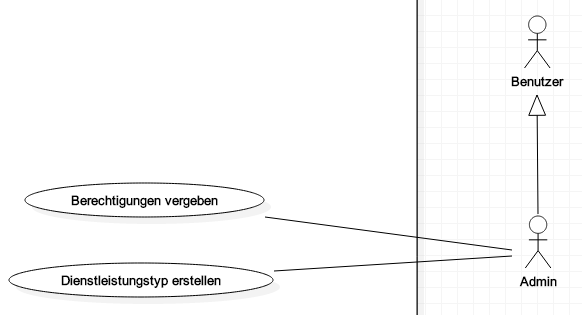
\includegraphics[width=.7\textwidth]{res/images/UseCaseAdmin.png}
\caption{Administrationsanforderungen}
\label{uc5}
\end{figure}

Als letztes zeigt die \myautoref{uc5} die Anforderungen der Administration an das System. Es sollen Funktionen vorgesehen werden, mit denen Berechtigungen an Benutzerkonten vergeben, wie auch Dienstleistungstypen angelegt werden können. Die Dienstleistungskategorien sollen nur von ausgewählten Benutzern angelegt bzw. editiert werden können, da sonst der Vorteil der Plattform, nämlich dass die Suche eines Anbieters bequem auf einen bestimmten Bereich eingeschränkt werden kann, nicht mehr gewährleistet werden kann.
